%%%%%%%%%%%%%%%%%%%%%%%%%%%%%%%%%%%%%%%%%
% Short Sectioned Assignment
% LaTeX Template
% Version 1.0 (5/5/12)
%
% This template has been downloaded from:
% http://www.LaTeXTemplates.com
%
% Original author:
% Frits Wenneker (http://www.howtotex.com)
%
% License:
% CC BY-NC-SA 3.0 (http://creativecommons.org/licenses/by-nc-sa/3.0/)
%
%%%%%%%%%%%%%%%%%%%%%%%%%%%%%%%%%%%%%%%%%

%----------------------------------------------------------------------------------------
%  PACKAGES AND OTHER DOCUMENT CONFIGURATIONS
%----------------------------------------------------------------------------------------

\documentclass[paper=a4, fontsize=12pt]{scrartcl}\usepackage{graphicx, color}
%% maxwidth is the original width if it is less than linewidth
%% otherwise use linewidth (to make sure the graphics do not exceed the margin)
\makeatletter
\def\maxwidth{ %
  \ifdim\Gin@nat@width>\linewidth
    \linewidth
  \else
    \Gin@nat@width
  \fi
}
\makeatother

\IfFileExists{upquote.sty}{\usepackage{upquote}}{}
\definecolor{fgcolor}{rgb}{0.2, 0.2, 0.2}
\newcommand{\hlnumber}[1]{\textcolor[rgb]{0,0,0}{#1}}%
\newcommand{\hlfunctioncall}[1]{\textcolor[rgb]{0.501960784313725,0,0.329411764705882}{\textbf{#1}}}%
\newcommand{\hlstring}[1]{\textcolor[rgb]{0.6,0.6,1}{#1}}%
\newcommand{\hlkeyword}[1]{\textcolor[rgb]{0,0,0}{\textbf{#1}}}%
\newcommand{\hlargument}[1]{\textcolor[rgb]{0.690196078431373,0.250980392156863,0.0196078431372549}{#1}}%
\newcommand{\hlcomment}[1]{\textcolor[rgb]{0.180392156862745,0.6,0.341176470588235}{#1}}%
\newcommand{\hlroxygencomment}[1]{\textcolor[rgb]{0.43921568627451,0.47843137254902,0.701960784313725}{#1}}%
\newcommand{\hlformalargs}[1]{\textcolor[rgb]{0.690196078431373,0.250980392156863,0.0196078431372549}{#1}}%
\newcommand{\hleqformalargs}[1]{\textcolor[rgb]{0.690196078431373,0.250980392156863,0.0196078431372549}{#1}}%
\newcommand{\hlassignement}[1]{\textcolor[rgb]{0,0,0}{\textbf{#1}}}%
\newcommand{\hlpackage}[1]{\textcolor[rgb]{0.588235294117647,0.709803921568627,0.145098039215686}{#1}}%
\newcommand{\hlslot}[1]{\textit{#1}}%
\newcommand{\hlsymbol}[1]{\textcolor[rgb]{0,0,0}{#1}}%
\newcommand{\hlprompt}[1]{\textcolor[rgb]{0.2,0.2,0.2}{#1}}%

\usepackage{framed}
\makeatletter
\newenvironment{kframe}{%
 \def\at@end@of@kframe{}%
 \ifinner\ifhmode%
  \def\at@end@of@kframe{\end{minipage}}%
  \begin{minipage}{\columnwidth}%
 \fi\fi%
 \def\FrameCommand##1{\hskip\@totalleftmargin \hskip-\fboxsep
 \colorbox{shadecolor}{##1}\hskip-\fboxsep
     % There is no \\@totalrightmargin, so:
     \hskip-\linewidth \hskip-\@totalleftmargin \hskip\columnwidth}%
 \MakeFramed {\advance\hsize-\width
   \@totalleftmargin\z@ \linewidth\hsize
   \@setminipage}}%
 {\par\unskip\endMakeFramed%
 \at@end@of@kframe}
\makeatother

\definecolor{shadecolor}{rgb}{.97, .97, .97}
\definecolor{messagecolor}{rgb}{0, 0, 0}
\definecolor{warningcolor}{rgb}{1, 0, 1}
\definecolor{errorcolor}{rgb}{1, 0, 0}
\newenvironment{knitrout}{}{} % an empty environment to be redefined in TeX

\usepackage{alltt} % A4 paper and 11pt font size

\usepackage[T1]{fontenc} % Use 8-bit encoding that has 256 glyphs
\usepackage{fourier} % Use the Adobe Utopia font for the document - comment this line to return to the LaTeX default
\usepackage[english]{babel} % English language/hyphenation
\usepackage{amsmath,amsfonts,amsthm} % Math packages

\usepackage{lipsum} % Used for inserting dummy 'Lorem ipsum' text into the template
\usepackage{pdfpages}
\usepackage{sectsty} % Allows customizing section commands
\allsectionsfont{ \normalfont\scshape} % Make all sections centered, the default font and small caps
\usepackage{algorithmic}
\usepackage{algorithm}
\usepackage{fancyhdr} % Custom headers and footers
\pagestyle{fancyplain} % Makes all pages in the document conform to the custom headers and footers
\fancyhead{} % No page header - if you want one, create it in the same way as the footers below
\fancyfoot[L]{} % Empty left footer
\fancyfoot[C]{} % Empty center footer
\fancyfoot[R]{\thepage} % Page numbering for right footer
\renewcommand{\headrulewidth}{0pt} % Remove header underlines
\renewcommand{\footrulewidth}{0pt} % Remove footer underlines
\setlength{\headheight}{13.6pt} % Customize the height of the header

\numberwithin{equation}{section} % Number equations within sections (i.e. 1.1, 1.2, 2.1, 2.2 instead of 1, 2, 3, 4)
\numberwithin{figure}{section} % Number figures within sections (i.e. 1.1, 1.2, 2.1, 2.2 instead of 1, 2, 3, 4)
\numberwithin{table}{section} % Number tables within sections (i.e. 1.1, 1.2, 2.1, 2.2 instead of 1, 2, 3, 4)

\setlength\parindent{1pt} % Removes all indentation from paragraphs - comment this line for an assignment with lots of text

%----------------------------------------------------------------------------------------
%	TITLE SECTION
%----------------------------------------------------------------------------------------

\newcommand{\horrule}[1]{\rule{\linewidth}{#1}} % Create horizontal rule command with 1 argument of height

\title{	
\normalfont \normalsize 
\textsc{Statistical Reservoir Modeling \\
(PETE 7285)} \\ [25pt] % Your university, school and/or department name(s)
\horrule{0.5pt} \\[0.4cm] % Thin top horizontal rule
\huge  Report \\ % The assignment title
\horrule{2pt} \\[0.5cm] % Thick bottom horizontal rule
}

\author{Esmail Ansari} % Your name

\date{\small\today} % Today's date or a custom date

\begin{document}

\maketitle % Print the title

%----------------------------------------------------------------------------------------
%	PROBLEM 1
%----------------------------------------------------------------------------------------

\section{Integrating models for facies prediction}

%-----------------------------------------
%----------------------------------------------------
%-------------
\subsection{Part A}
The course codes were trimmed so that they only output scaled kapur data (function \texttt{scaleKapur}). Then, the kapur facies are counted using \texttt{table} function and probability (proportion) of each facies is computed. 

\begin{knitrout}
\definecolor{shadecolor}{rgb}{0.969, 0.969, 0.969}\color{fgcolor}\begin{kframe}
\begin{alltt}
\hlcomment{#cleaning variables and closing plots}
\hlfunctioncall{rm}(list=\hlfunctioncall{ls}())
\hlfunctioncall{if} (!\hlfunctioncall{is.null}(\hlfunctioncall{dev.list}())) \hlfunctioncall{dev.off}()

\hlcomment{#loading packages}
\hlfunctioncall{require}(boot)
\hlfunctioncall{require}(nnet)
\hlfunctioncall{require}(RColorBrewer)
\hlfunctioncall{require}(ggplot2)
\hlfunctioncall{require}(lattice)
line.colors <- \hlfunctioncall{brewer.pal}(N.facies,\hlstring{"Dark2"})

\hlcomment{#Counting facies using 'table' function}
facies     = kapur[\hlstring{"facies"}]
tab.facies = \hlfunctioncall{table}(facies)
N.facies   = \hlfunctioncall{length}(tab.facies)
tot.obs    = \hlfunctioncall{sum}(tab.facies)
p.facies   = tab.facies/tot.obs
\end{alltt}
\end{kframe}
\end{knitrout}


For fitting a beta distribution to the facies, the total counts are used for estimating alpha and beta. \texttt{dbeta} function is then used for calculating the probability of facies proportions. The results are then tabulated to be used by \textit{lattice} package. 

\begin{knitrout}
\definecolor{shadecolor}{rgb}{0.969, 0.969, 0.969}\color{fgcolor}\begin{kframe}
\begin{alltt}
\hlfunctioncall{for} (i in 1:N.facies)\{
\hlcomment{  #evaluating the parameters of beta function and facies pdf}
  x     =  \hlfunctioncall{seq}(0,1,0.001)
  alpha = tab.facies+1
  beta  =  tot.obs-tab.facies+1
  p.df  = \hlfunctioncall{dbeta}(x,alpha[i],beta[i])
  
\hlcomment{  #tidy up for lattice package }
  current.size = \hlfunctioncall{length}(x)
  sum.size.pri = current.size+sum.size.pri
  all.prior[(sum.size.pri-current.size):(sum.size.pri-1),1] = x
  all.prior[(sum.size.pri-current.size):(sum.size.pri-1),2] = 
    p.df/\hlfunctioncall{sum}(p.df)
  all.prior[(sum.size.pri-current.size):(sum.size.pri-1),3] =
   \hlfunctioncall{rep}(\hlfunctioncall{paste}(\hlstring{"facies "},i),\hlfunctioncall{length}(x))    
\}
\hlcomment{#plotting priors using lattice package }
line.colors = \hlfunctioncall{brewer.pal}(N.facies,\hlstring{"Dark2"})
myStrip     = \hlfunctioncall{function}(which.panel, factor.levels, ...) \{
  \hlfunctioncall{panel.rect}(0, 0, 1, 1,col = line.colors[which.panel],border = 1)
  \hlfunctioncall{panel.text}(x = 0.5, y = 0.5,font = 2,lab = factor.levels[which.panel])
\}
\hlfunctioncall{print}(\hlfunctioncall{xyplot}(Probability ~ Proportion|Facies.type,
               data = all.prior[1:sum.size.pri-1,],
               type = \hlstring{"l"},lwd = 3,strip = myStrip))
\end{alltt}
\end{kframe}
\end{knitrout}



%-------------
\subsection{Part B}
Function \texttt{prob.facies} was prepared for bootstraping using \texttt{boot} function. This function fits the multinomial regression to the facies and outputs the probability of probability of each facies. 
\begin{knitrout}
\definecolor{shadecolor}{rgb}{0.969, 0.969, 0.969}\color{fgcolor}\begin{kframe}
\begin{alltt}
\hlcomment{#Defining the probability function to be bootstrapped}
prob.facies     <-  \hlfunctioncall{function}(formula, data, indices)\{
  selected.data   =  data[indices,]
  kapur.glm       =  \hlfunctioncall{multinom}(formula,data=selected.data)
  pred.glm        =  \hlfunctioncall{fitted}(kapur.glm)
  pred.glm        =  \hlfunctioncall{sortPredByLevels}(pred.glm)
  most.likely.glm =  \hlfunctioncall{apply}(pred.glm,1,which.max)
  tab.pred.facies =  \hlfunctioncall{table}(most.likely.glm)
  tot.obs         =   \hlfunctioncall{sum}(tab.pred.facies)
  all.fac.name    =  \hlfunctioncall{names}(\hlfunctioncall{table}(data$facies))
  N.facies        =   \hlfunctioncall{length}(all.fac.name)
  idxToFac        =   all.fac.name
  \hlfunctioncall{names}(idxToFac) =   \hlfunctioncall{as.character}(1:N.facies)
  sel.fac.name    =   \hlfunctioncall{names}(tab.pred.facies)
  \hlfunctioncall{names}(tab.pred.facies) = idxToFac[sel.fac.name]
  no.occur.facies =   \hlfunctioncall{setdiff}(all.fac.name,sel.fac.name)
  prob            =   \hlfunctioncall{rep}(NA,N.facies)
  \hlfunctioncall{names}(prob)     =  all.fac.name
  \hlfunctioncall{if} (\hlfunctioncall{any}(\hlfunctioncall{as.integer}(no.occur.facies))) \{
    prob[no.occur.facies] = 0
  \}
  prob[sel.fac.name]  =  \hlfunctioncall{as.vector}(tab.pred.facies)/tot.obs
\hlfunctioncall{return}(prob)
\}
\end{alltt}
\end{kframe}
\end{knitrout}


Note that when we are using bootstraping for categorical data, we face two important challenges. First, some facies type may not be sampled and second some facies type may not be predicted. For both of these situations we should put the probability of such facies to zero. Here, facies 2 and 7 occur relatively few times and sometimes they may not be sampled or predictred. Below lines (which are in \texttt{prob.facies} function) are added for detecting unsampled facies and enforcing their probabilities as zero when bootstapping. Below chunck demonstrates the idea of naming  existing facies according to the indeices that come out of \texttt{which.max} function.

\begin{knitrout}
\definecolor{shadecolor}{rgb}{0.969, 0.969, 0.969}\color{fgcolor}\begin{kframe}
\begin{alltt}
all.fac.name    =  \hlfunctioncall{names}(\hlfunctioncall{table}(data$facies))
N.facies        =   \hlfunctioncall{length}(all.fac.name)
idxToFac        =   all.fac.name
\hlfunctioncall{names}(idxToFac) =   \hlfunctioncall{as.character}(1:N.facies)
sel.fac.name    =   \hlfunctioncall{names}(tab.pred.facies)
\hlfunctioncall{names}(tab.pred.facies) = idxToFac[sel.fac.name]
no.occur.facies =   \hlfunctioncall{setdiff}(all.fac.name,sel.fac.name)
prob            =   \hlfunctioncall{rep}(NA,N.facies)
\hlfunctioncall{names}(prob)     =  all.fac.name
\hlfunctioncall{if} (\hlfunctioncall{any}(\hlfunctioncall{as.integer}(no.occur.facies))) \{
  prob[no.occur.facies] = 0 
\end{alltt}
\end{kframe}
\end{knitrout}


And finally function \texttt{prob.facies} is prepared to be passed to  function \texttt{boot} to be bootstrapped 300 times. 

\begin{knitrout}
\definecolor{shadecolor}{rgb}{0.969, 0.969, 0.969}\color{fgcolor}\begin{kframe}
\begin{alltt}
\hlcomment{# Bootstrapping using boot function}
form        = facies ~ caliper + ind.deep + gamma + r.deep + density

boot.result = \hlfunctioncall{boot}(formula=form, statistic=prob.facies,
                   data=\hlfunctioncall{scaleKapur}(kapur),R=N.Boot)
\end{alltt}
\end{kframe}
\end{knitrout}


%-------------
\subsection{Part C}
Posteriors are calculated by multiplying the priors and likelihoods. In below code \texttt{y} represents the likelihood and \texttt{p.df} represents the prior counts for the facies. 
\begin{knitrout}
\definecolor{shadecolor}{rgb}{0.969, 0.969, 0.969}\color{fgcolor}\begin{kframe}
\begin{alltt}
\hlcomment{# Finding and plotting facies posteriors}
posterior = p.df * y/\hlfunctioncall{sum}(p.df * y)
\end{alltt}
\end{kframe}
\end{knitrout}

and then we plot the posterior of each facies using 
\textit{ggplot2} package. 
\begin{knitrout}
\definecolor{shadecolor}{rgb}{0.969, 0.969, 0.969}\color{fgcolor}\begin{kframe}
\begin{alltt}
  df       = \hlfunctioncall{data.frame}(x,prior,likelihood,posterior)
  
  g[[i]]   = \hlfunctioncall{ggplot}( df, \hlfunctioncall{aes}(x)) +                   
                    \hlfunctioncall{geom_line}(\hlfunctioncall{aes}(y=prior,colour=\hlstring{"prior"})) +  
                    \hlfunctioncall{geom_line}(\hlfunctioncall{aes}(y=likelihood,colour=\hlstring{"likelihood"})) +  
                    \hlfunctioncall{geom_line}(\hlfunctioncall{aes}(y=posterior,colour=\hlstring{"posterior"}) )
  
  g[[i]]  = g[[i]] + \hlfunctioncall{xlab}(\hlfunctioncall{paste}(\hlstring{"proportion of facies "}, 
                     \hlfunctioncall{names}(tab.facies[i]))) + \hlfunctioncall{ylab}(\hlstring{"Probability"})+
                     \hlfunctioncall{scale_colour_manual}(\hlstring{""},values=\hlfunctioncall{c}(\hlstring{"darkgreen"},\hlstring{"blue"},\hlstring{"red"}))


\hlfunctioncall{require}(gridExtra)
\hlfunctioncall{for} (i in \hlfunctioncall{seq}(1,8,2))\{
  sidebysideplot = \hlfunctioncall{grid.arrange}(g[[i]], g[[i+1]], nrow=2)
  \hlfunctioncall{print}(sidebysideplot)
\}
\end{alltt}
\end{kframe}
\end{knitrout}

For facies 1 and 2, the likelihood improves our belief about the proportion of these facies and our model strengthens the priors. The likelihood weakens our confidence (prior) on probabilities of facies 5 and 7. Probabilities of facies 9 and 10 are not affected using bayesian analysis. This may be because their proportions are already high and likelihood also approves the priors to be the best representation of these facies. For facies 3, the likelihood hugely changes our understanding of it's probability. It inidcates that most probable proportion of facies 3 is 0.055 and our prior opinion of 0.07 may not be accurate based on new evidence (bootstrapped multinomial model). 


\begin{figure}[htbp]
\begin{center}
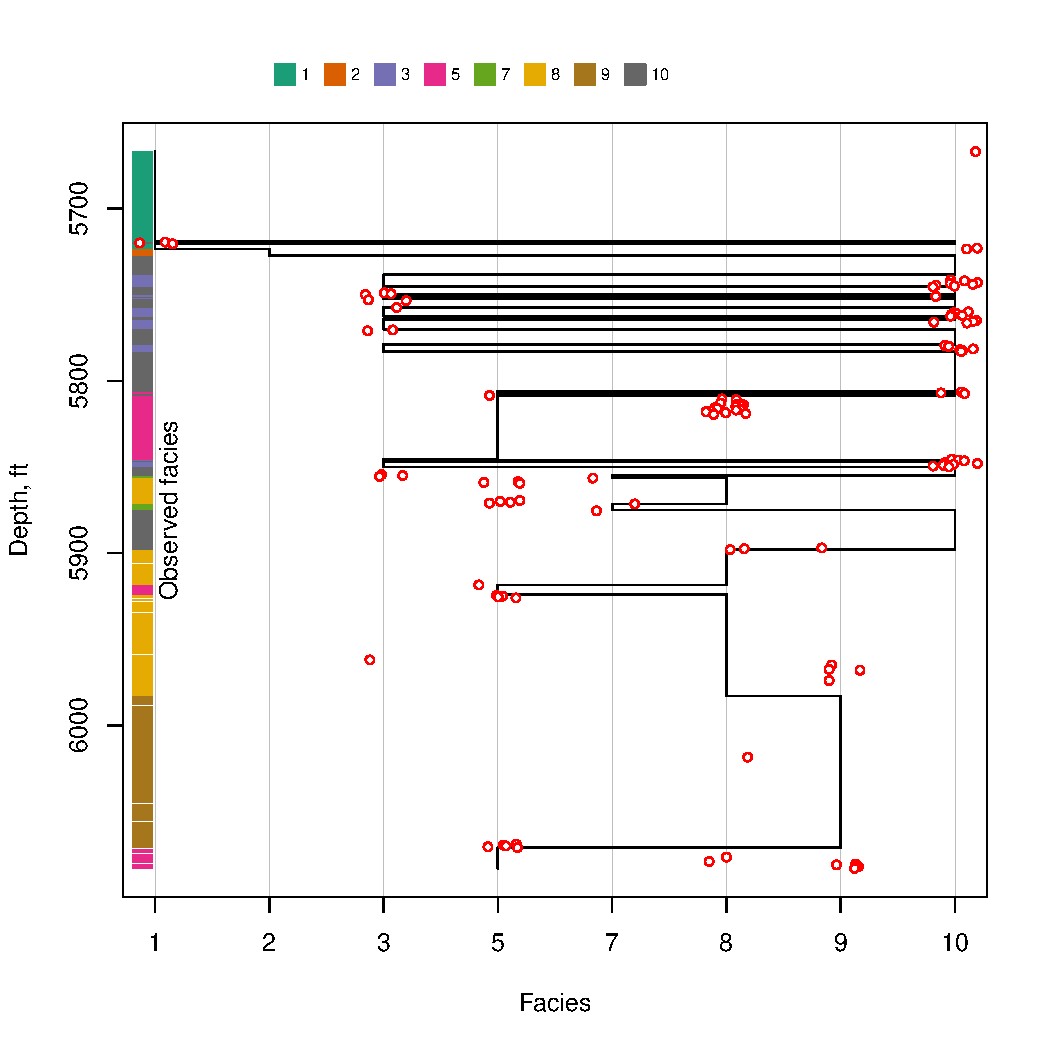
\includegraphics[width=\linewidth]{LDAfit.pdf}
\caption{we just used linear discrimentant analysis instead of logistic regression to plot prediction vs. depth. Posteriors are not used in constructing this figure.}
\label{simPlot}
\end{center}
\end{figure}

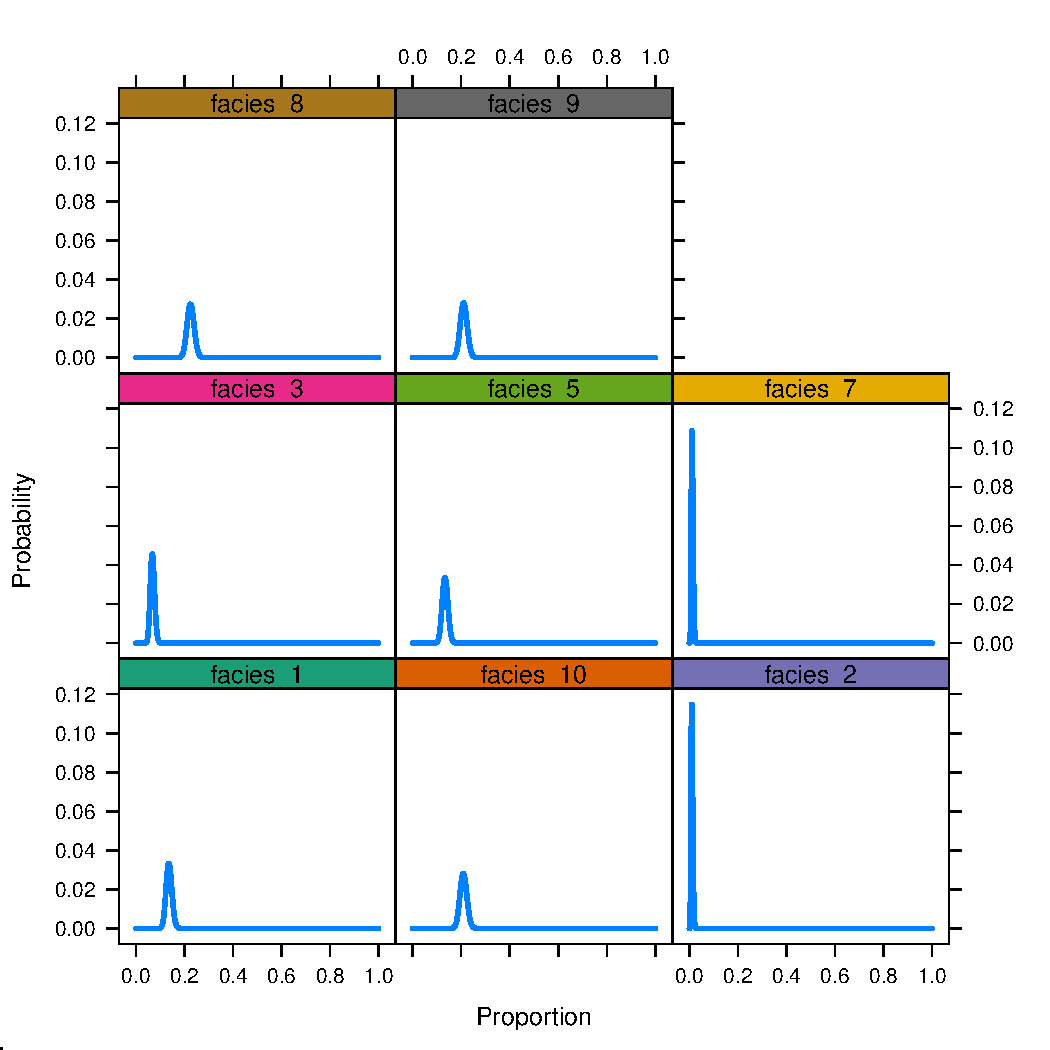
\includepdf[pages={1,2}]{prior-likelihood.pdf}

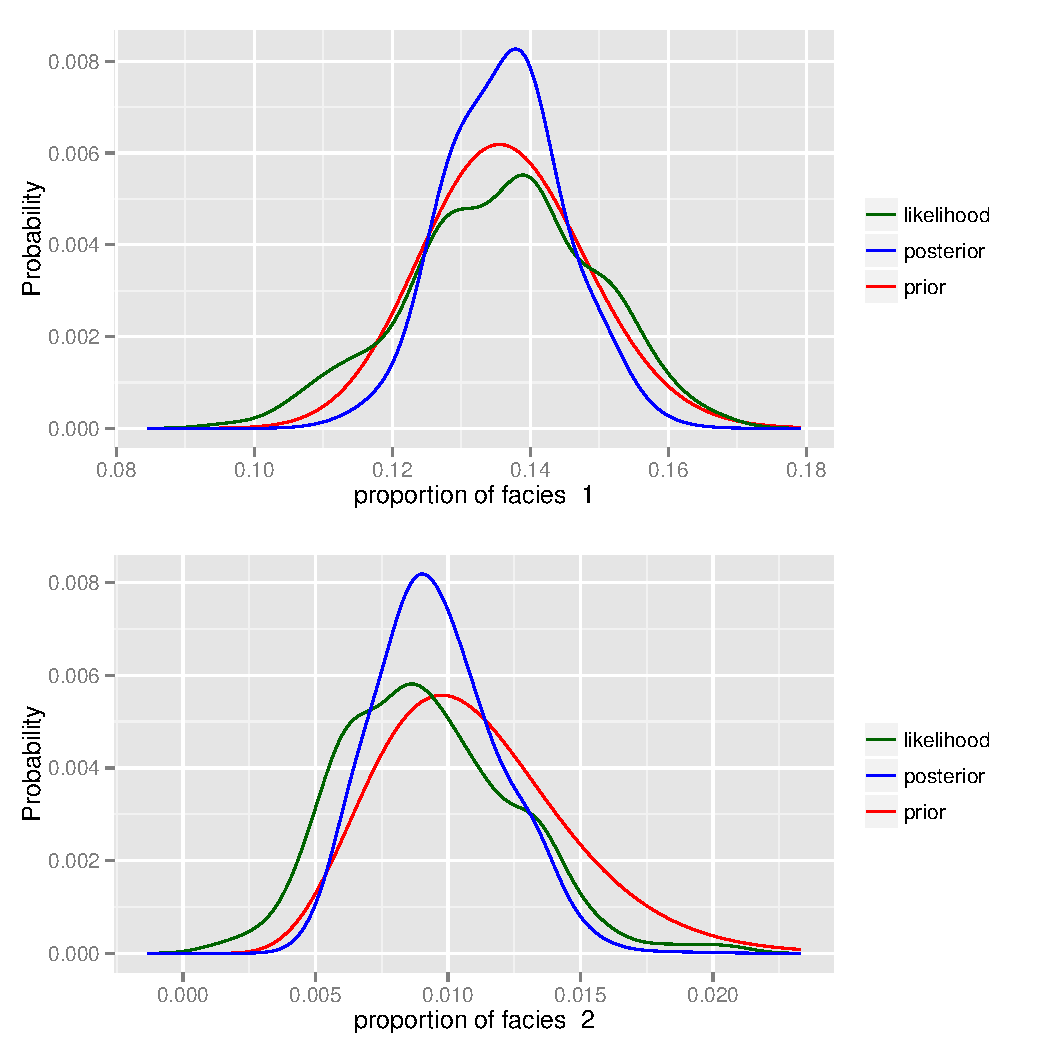
\includepdf[pages={1,2,3,4},width=1.2\linewidth]{posterior.pdf}


%--------------
%%%PROBLEM 2
%---------------------
\section{Markov chain as a stochastic graph}
%-------------
Various assumptions used for solving this problem are summarized below. 
\begin{enumerate}
\item For the work over, first arrived well, will be served first.
\item If multiple well damage at the same time, the oldest well(the well that has started the chain sooner) will be worked over first. 
\item The reservoir engineer has estimated a value of N.true for each well. As soon as this value becomes zero (or less), the well is considered depleted and should be abandoned. 
\item For constructing violin plot, only drilling risks are taken into consideration and reserovir engineer's prediction (N.true) will remain the same for all runs. If desired, this assumption can be easily eleminated.   
\end{enumerate}

\texttt{SetState.R} contains functions that make small changes to state transitions. 
\begin{knitrout}
\definecolor{shadecolor}{rgb}{0.969, 0.969, 0.969}\color{fgcolor}\begin{kframe}
\begin{alltt}
\hlcomment{#Defining states, costs and state transition functions}
\hlfunctioncall{rm}(list=\hlfunctioncall{ls}())
\hlfunctioncall{source}(\hlfunctioncall{file.path}(\hlstring{'/Users/eansar2/Desktop/Geostatistics/TakeHome'},
                 \hlstring{'SetState.R'}))
costs <- \hlfunctioncall{list}(Queue=0,Drill=-25,FinishedDrill=0,Complete=-25,Produce=-0.1,
              Shut_in=0,WaitForRig=0,WorkOver=-25,Abandon=-10)
states <-   \hlfunctioncall{c}(\hlstring{"Queue"},\hlstring{"Drill"},\hlstring{"FinishedDrill"},\hlstring{"Complete"},\hlstring{"Produce"},
              \hlstring{"Shut_in"},\hlstring{"WaitForRig"},\hlstring{"WorkOver"},\hlstring{"Abandon"})

\end{alltt}
\end{kframe}
\end{knitrout}


%---algorithm
 \begin{algorithm}
 \caption{Markov Chain}
 \label{alg1}
 \begin{algorithmic}[1]
 \STATE Initialize variables
 \WHILE{not all wells abandoned}
 \FOR{each wells}
 \IF{drilling job finished}
 \STATE Move the well out of drilling state
 \ENDIF
 \IF{drilling is empty and this well is in queue}
 \STATE Drill this well
 \ENDIF
 \IF{any well is damaged}
 \STATE Work over the earlier damaged well (oldest if multiple)
 \ENDIF
 \STATE Determine the next state of the well
 \ENDFOR
 \FOR{all wells}
 \STATE Update the well's current state and adjust it's properties
 \STATE calculate the profit
 \STATE calculate N.ture
 \IF{N.true<=0}
 \STATE flag the well for abandoning 
 \ENDIF
 \IF{any well is in wait for rig state}
 \STATE determine possible workover wells and select only one based on assumptions
 \ENDIF
 \ENDFOR
 \STATE time=time+1
 \ENDWHILE
 \end{algorithmic}
 \end{algorithm}
%-------
Three additional properties (\texttt{current.state, next.state, drilling.flag}) are added to the course notes proposed well objects in order to track them more easily. All wells are in Queue at the begining \textit(time zero). 
\begin{knitrout}
\definecolor{shadecolor}{rgb}{0.969, 0.969, 0.969}\color{fgcolor}\begin{kframe}
\begin{alltt}
\hlcomment{#Initializing well objects}
wells <- \hlfunctioncall{vector}(\hlstring{"list"},N.wells)
\hlfunctioncall{for} (i in 1:N.wells)\{
  wells[[i]] = \hlfunctioncall{list}(current.state=\hlstring{"Queue"},next.state=\hlstring{"Queue"},
                    t.states=\hlfunctioncall{matrix}(0,10000,N.states),
                    t.drill=\hlfunctioncall{sample}(2:6,1,p=\hlfunctioncall{c}(0,0.25,0.5,0.75,1)),
                    t.this=0,N.believe=\hlfunctioncall{runif}(1,500,1000),
                    N.true=\hlfunctioncall{runif}(1,500,1000),q=\hlfunctioncall{runif}(1,0.5,3),value=0,
                    drilling.flag=FALSE)
  
  \hlfunctioncall{colnames}(wells[[i]]$t.states) <- states
\}
\end{alltt}
\end{kframe}
\end{knitrout}

Initialize the transition matrix so that all the pathes between states are open at the begining. 
\begin{knitrout}
\definecolor{shadecolor}{rgb}{0.969, 0.969, 0.969}\color{fgcolor}\begin{kframe}
\begin{alltt}
\hlcomment{#Defining initial transition matrix }
trans.prob = \hlfunctioncall{matrix}(0,nrow=N.states,ncol=N.states,
                    dimnames=\hlfunctioncall{list}(states,states))
trans.prob = \hlfunctioncall{initialize}(trans.prob) \hlcomment{#initializing transition matrix}
\end{alltt}
\end{kframe}
\end{knitrout}

\texttt{Drilling.flag} shows which well is being drilled. \texttt{wells.abandoned} records the wells that are absorbed. 
\begin{knitrout}
\definecolor{shadecolor}{rgb}{0.969, 0.969, 0.969}\color{fgcolor}\begin{kframe}
\begin{alltt}
\hlcomment{#Initiallizing variables}
drilling.flag      = \hlfunctioncall{rep}(FALSE,N.wells)
wells.abandoned    = \hlfunctioncall{rep}(FALSE,N.wells)
pos.workover.wells = \hlfunctioncall{rep}(FALSE,N.wells)
def.N.true.wells   = \hlfunctioncall{rep}(FALSE,N.wells)
waiting.time       = \hlfunctioncall{rep}(0,N.wells)
workover.well      = 0
time               = 0
\end{alltt}
\end{kframe}
\end{knitrout}

It is not necessary, but would be more understandable and sometimes useful, if we calculate the costs and some other paramters in a separate \texttt{for} loop. (i.e. after all wells are moved one step and before the end of the month). 
\begin{knitrout}
\definecolor{shadecolor}{rgb}{0.969, 0.969, 0.969}\color{fgcolor}\begin{kframe}
\begin{alltt}
\hlcomment{#Main loop }
\hlfunctioncall{while} (!\hlfunctioncall{all}(wells.abandoned))\{
\hlcomment{   #First for loop}
   \hlfunctioncall{for} (i in 1:N.wells)\{
\hlcomment{     #move wells one time step}
     ...
   \}
\hlcomment{   #Second for loop}
   \hlfunctioncall{for} (i in 1:N.wells)\{
\hlcomment{     #for calculating the costs }
     ...
   \}   
  ...
  wells.abandoned[[i]] = (wells[[i]]$current.state==\hlstring{"Abandon"})
  time=time+1 
\}
\end{alltt}
\end{kframe}
\end{knitrout}

The next state is sampled between all posible pathes weighted by their probabilities.
\begin{knitrout}
\definecolor{shadecolor}{rgb}{0.969, 0.969, 0.969}\color{fgcolor}\begin{kframe}
\begin{alltt}
\hlcomment{    #select the next state.}
    pos.next.states <- \hlfunctioncall{names}(\hlfunctioncall{which}(  trans.prob[current.state,]!=0 )) 
    prob.next.states  <- trans.prob[current.state,pos.next.states]
    selected.next.state <- \hlfunctioncall{sample}(pos.next.states,1,p=prob.next.states)
    wells[[i]]$next.state <- selected.next.state
\end{alltt}
\end{kframe}
\end{knitrout}

Below chunck demonstrates how workover wells are selected. 
\begin{knitrout}
\definecolor{shadecolor}{rgb}{0.969, 0.969, 0.969}\color{fgcolor}\begin{kframe}
\begin{alltt}
\hlcomment{  #In the second "for" loop}
    pos.workover.wells[i]=(wells[[i]]$current.state==\hlstring{"WaitForRig"})
    waiting.time[i] = \hlfunctioncall{as.integer}(pos.workover.wells[i])
                      *wells[[i]]$t.this

\hlcomment{  #Before increasing time step, check for workover wells}
  \hlfunctioncall{if} (\hlfunctioncall{any}(pos.workover.wells))
  \{
\hlcomment{    #First check which wells have arrived at WaitForRig state}
    max.waiting.wells = \hlfunctioncall{which}(waiting.time==
                              \hlfunctioncall{max}(waiting.time[pos.workover.wells]))
    
\hlcomment{    #If more than one well arrive at the same time, choose the well}
\hlcomment{    # has started the chain sooner(Oldest well)}
    workover.well     = \hlfunctioncall{min}(max.waiting.wells)  
  \}else\{
    workover.well     = 0
  \}
\end{alltt}
\end{kframe}
\end{knitrout}

Below chunck is located at the begining of the first \texttt{for} loop to check whether the drilling state is empty. 

\begin{knitrout}
\definecolor{shadecolor}{rgb}{0.969, 0.969, 0.969}\color{fgcolor}\begin{kframe}
\begin{alltt}
\hlcomment{    #check if any well is being drilled. If not, the next well can be}
\hlcomment{    #drilled. }
    \hlfunctioncall{for} (j in 1:N.wells)
       drilling.flag[j] =wells[[j]]$drilling.flag   
    \hlfunctioncall{if} (\hlfunctioncall{any}(drilling.flag))
        trans.prob <- \hlfunctioncall{drill.close}(trans.prob) else
        trans.prob <- \hlfunctioncall{drill.open}(trans.prob)
\end{alltt}
\end{kframe}
\end{knitrout}

The below code is added for abandoning depleted wells. 
\begin{knitrout}
\definecolor{shadecolor}{rgb}{0.969, 0.969, 0.969}\color{fgcolor}\begin{kframe}
\begin{alltt}
\hlcomment{     #If N.true of the well is depleted, abandon that well. }
     def.N.true.wells[i] = (wells[[i]]$N.true <= 0)
     \hlfunctioncall{if} (def.N.true.wells[i])
        trans.prob <- \hlfunctioncall{well.abandon}(trans.prob)  else 
        trans.prob <- \hlfunctioncall{well.open}(trans.prob)
\end{alltt}
\end{kframe}
\end{knitrout}

Below code is for moving the well out of the drilling state into the finished drilling state if it's \texttt{t.drill} is fulfilled.
\begin{knitrout}
\definecolor{shadecolor}{rgb}{0.969, 0.969, 0.969}\color{fgcolor}\begin{kframe}
\begin{alltt}
\hlcomment{     #If drilling is finished move the well out. }
     \hlfunctioncall{if} (\hlfunctioncall{sum}(wells[[i]]$t.states[,\hlstring{"Drill"}])==wells[[i]]$t.drill)
        trans.prob <- \hlfunctioncall{Finished.drill.open}(trans.prob) else
        trans.prob <- \hlfunctioncall{Finished.drill.close}(trans.prob)

\end{alltt}
\end{kframe}
\end{knitrout}

Below chunck should be clear. 
\begin{knitrout}
\definecolor{shadecolor}{rgb}{0.969, 0.969, 0.969}\color{fgcolor}\begin{kframe}
\begin{alltt}
\hlcomment{     #WorkOver is only open for one well at time}
     \hlfunctioncall{if} (i==workover.well)
        trans.prob <- \hlfunctioncall{WorkOver.open}(trans.prob) else 
        trans.prob <- \hlfunctioncall{WorkOver.close}(trans.prob)
\end{alltt}
\end{kframe}
\end{knitrout}

And finally the costs are calculated in the second \texttt{for} loop.
\begin{knitrout}
\definecolor{shadecolor}{rgb}{0.969, 0.969, 0.969}\color{fgcolor}\begin{kframe}
\begin{alltt}
\hlcomment{    #calculate the profit and modify the value of the well}
    profit=\hlfunctioncall{as.integer}(wells[[i]]$current.state==\hlstring{"Produce"})*wells[[i]]$q
    \hlfunctioncall{if} (!(wells[[i]]$current.state==\hlstring{"Abandon"}))
      wells[[i]]$value = (wells[[i]]$value+
                          costs[[wells[[i]]$current.state]]+profit)
\hlcomment{    #The cost of Abandon state is single time cost. }
    \hlfunctioncall{if} ((wells[[i]]$current.state==\hlstring{"Abandon"})&&(wells[[i]]$t.this==1))
      wells[[i]]$value = (wells[[i]]$value+
                          costs[[wells[[i]]$current.state]]+profit)
\end{alltt}
\end{kframe}
\end{knitrout}


Log of the wells for a prolific field development (revenue of around $2100$ million \$ after all wells are abandoned) are shown below. As violen plot indicates this is one of the profitable develpments. The average revenue (after 1000 months) is around 600 million \$. 

%\begin{figure}[htbp]
%\begin{center}
%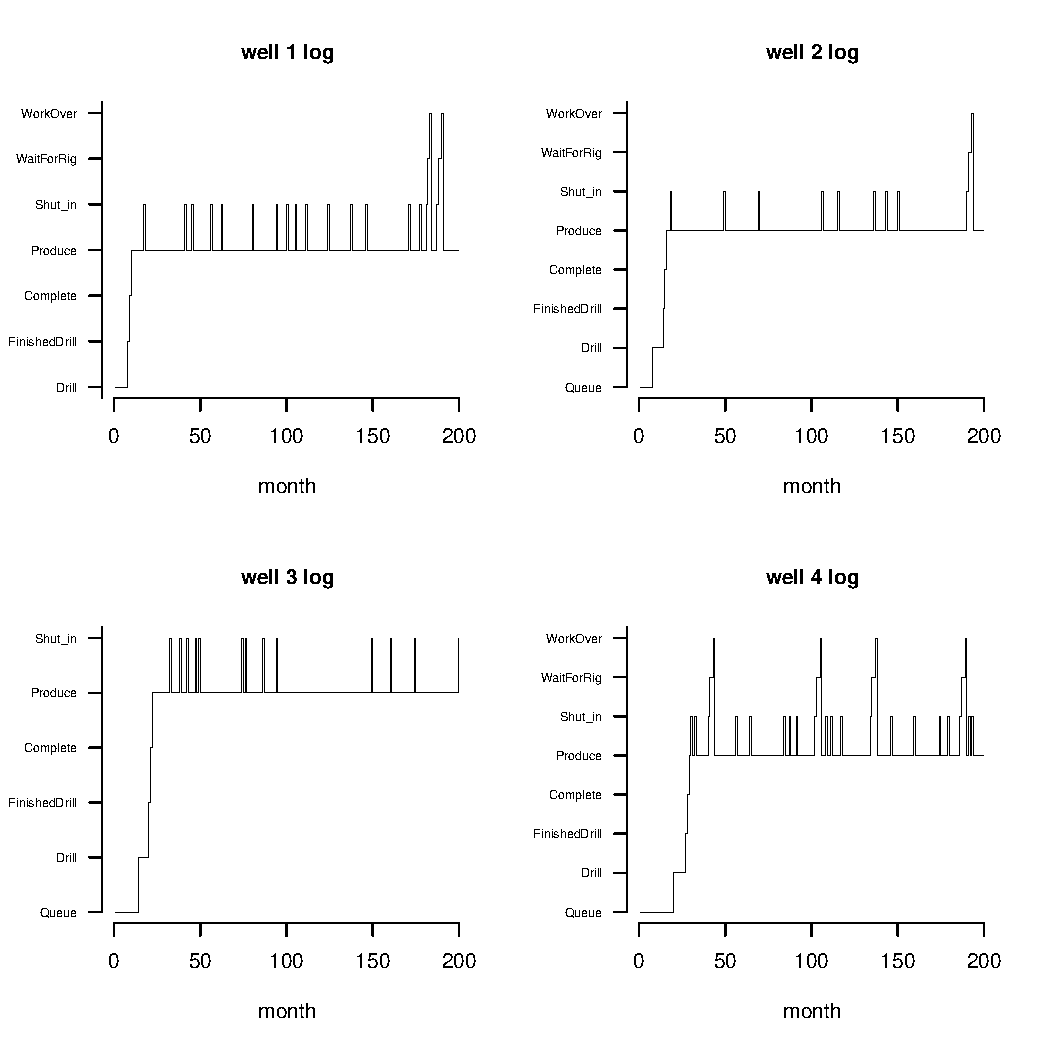
\includepdf[pages={1}]{simulationPlot.pdf}
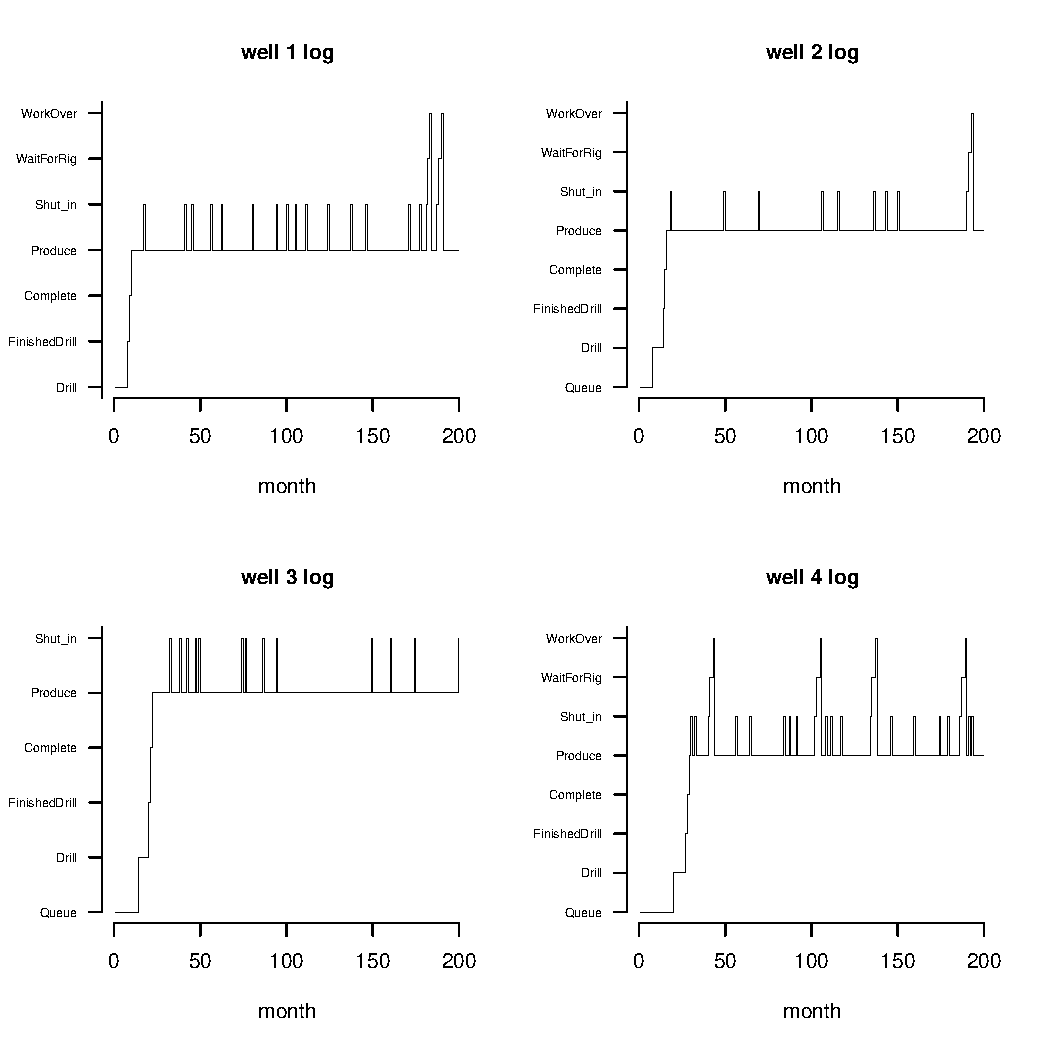
\includepdf[pages={1,2,3}]{simulationPlot.pdf}
\pagebreak
%\caption{}
% \label{simPlot}
%\end{center}
%\end{figure}


\begin{figure}[htbp]
\begin{center}
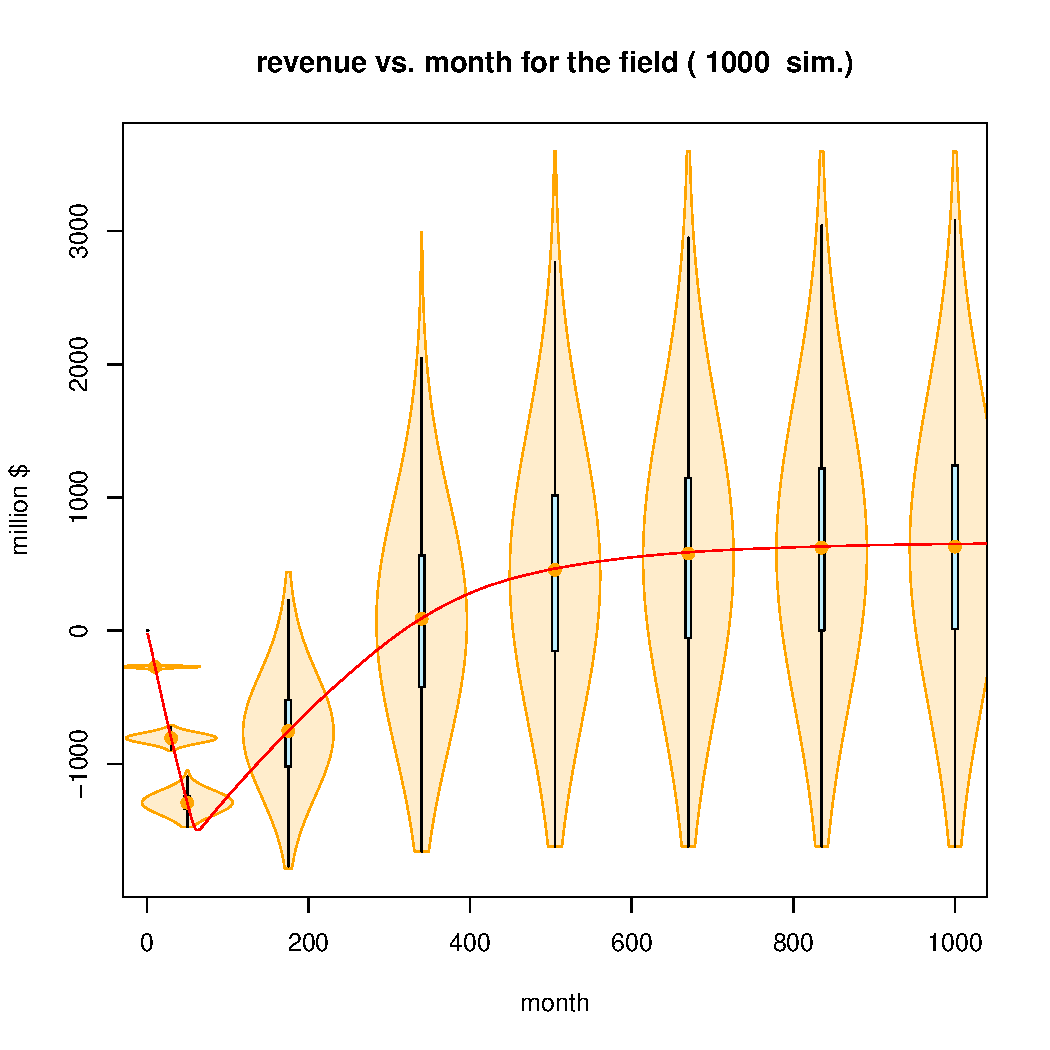
\includegraphics[width=\linewidth]{vioplot.pdf}
\caption{Violin plot for the field develpment. The red line connects the mean of field net revenue calculated after each month. It turns out that the mean is equal to the median. The skewness of the kernell densities for all months are small and upward. It is more likely that we have to wait around 300 months to get our investment money back. If we are the most luckiest person on earth, this waiting time would decrease to 180 months and 3800 million \$ is the maximum revenue we will attain. The most probable maximum cost would be around 1500 million and it happens after around 70 months. The maximum amount that we have to invest on field development does not depend (relatively) on whether we are lucky or not. After a $1000$ month!($83$ years), the $0.25$ percent quantile of violins are roughly higher than zero which can be promising if we are interested in long term revenue. 
}
\label{simPlot}
\end{center}
\end{figure}


%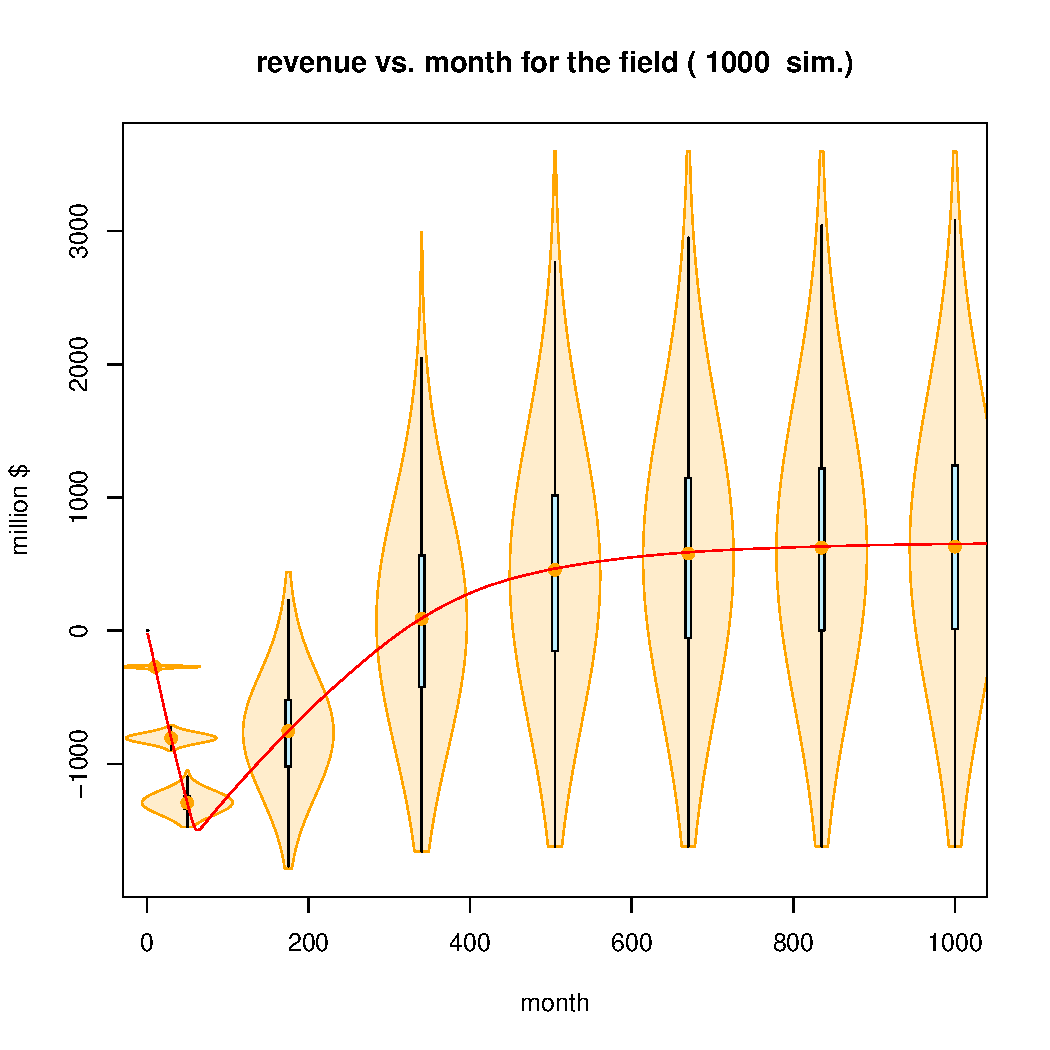
\includepdf[pages={1},width=1\linewidth]{vioplot.pdf}

\end{document}
